%%%%%%%% CIL 2024 EXAMPLE LATEX SUBMISSION FILE %%%%%%%%%%%%%%%%%

% This template was adopted from the ICML 2024 tempalte!

\documentclass{article}

% Recommended, but optional, packages for figures and better typesetting:
\usepackage{microtype}
\usepackage{graphicx}
\usepackage{subfigure}
\usepackage{booktabs} % for professional tables
\usepackage{hyperref}
\usepackage{algorithm2e}
\usepackage{adjustbox}

% Attempt to make hyperref and algorithmic work together better:
\newcommand{\theHalgorithm}{\arabic{algorithm}}
\usepackage[accepted]{icml2024}

% For theorems and such
\usepackage{amsmath}
\usepackage{amssymb}
\usepackage{mathtools}
\usepackage{amsthm}

% if you use cleveref..
\usepackage[capitalize,noabbrev]{cleveref}

\usepackage{amsmath,amssymb,amsfonts}
\usepackage{graphicx}
\usepackage{textcomp}
\usepackage{xcolor}
\usepackage{float}
\usepackage{booktabs}

\usepackage{tikz}
\usepackage{pgfplots}
\pgfplotsset{compat=1.17}
\def\BibTeX{{\rm B\kern-.05em{\sc i\kern-.025em b}\kern-.08em
    T\kern-.1667em\lower.7ex\hbox{E}\kern-.125emX}}

\usepackage{tikz}
\usetikzlibrary{positioning, shapes.geometric, arrows.meta}

\definecolor{customBar}{HTML}{F2AA84} 

%\newcommand{\theHalgorithm}{\arabic{algorithm}}

%%%%%%%%%%%%%%%%%%%%%%%%%%%%%%%%
% THEOREMS
%%%%%%%%%%%%%%%%%%%%%%%%%%%%%%%%
\theoremstyle{plain}
\newtheorem{theorem}{Theorem}[section]
\newtheorem{proposition}[theorem]{Proposition}
\newtheorem{lemma}[theorem]{Lemma}
\newtheorem{corollary}[theorem]{Corollary}
\theoremstyle{definition}
\newtheorem{definition}[theorem]{Definition}
\newtheorem{assumption}[theorem]{Assumption}
\theoremstyle{remark}
\newtheorem{remark}[theorem]{Remark}

% Todonotes is useful during development; simply uncomment the next line
%    and comment out the line below the next line to turn off comments
%\usepackage[disable,textsize=tiny]{todonotes}
\usepackage[textsize=tiny]{todonotes}

% Math Macros
\DeclareMathOperator*{\argmin}{arg\,min}
\DeclareMathOperator*{\argmax}{arg\,max}
\DeclareMathOperator*{\topK}{topK}
\DeclareMathOperator*{\flopK}{flopK}

% Colors
\definecolor{ourorange}{HTML}{B25628}
\definecolor{ourblue}{HTML}{2A749E}


% The \icmltitle you define below is probably too long as a header.
% Therefore, a short form for the running title is supplied here:
\icmltitlerunning{Learned Prompting for Sentiment Analysis with LLMs}

\begin{document}

\twocolumn[
\icmltitle{Learned Prompting for Sentiment Analysis with LLMs}

% It is OKAY to include author information, even for blind
% submissions: the style file will automatically remove it for you
% unless you've provided the [accepted] option to the icml2024
% package.

% List of affiliations: The first argument should be a (short)
% identifier you will use later to specify author affiliations
% Academic affiliations should list Department, University, City, Region, Country
% Industry affiliations should list Company, City, Region, Country

% You can specify symbols, otherwise they are numbered in order.
% Ideally, you should not use this facility. Affiliations will be numbered
% in order of appearance and this is the preferred way.
\icmlsetsymbol{equal}{*}

\begin{icmlauthorlist}
\icmlauthor{Niklas Britz  }{}
\icmlauthor{Karl Deck  }{}
\icmlauthor{Marie-Louise Dugua  }{}
\icmlauthor{Alexander Zank  }{}
\end{icmlauthorlist}

%\icmlaffiliation{eth}{Department of Computer Science, ETH Zürich, Zürich, Switzerland}
%\icmlaffiliation{comp}{Company Name, Location, Country}
%\icmlaffiliation{sch}{School of ZZZ, Institute of WWW, Location, Country}

\icmlcorrespondingauthor{Firstname1 Lastname1}{first1.last1@xxx.edu}
\icmlcorrespondingauthor{Firstname2 Lastname2}{first2.last2@www.uk}

% You may provide any keywords that you
% find helpful for describing your paper; these are used to populate
% the "keywords" metadata in the PDF but will not be shown in the document
\icmlkeywords{Machine Learning, ICML}

\vskip 0.3in
]

% this must go after the closing bracket ] following \twocolumn[ ...

% This command actually creates the footnote in the first column
% listing the affiliations and the copyright notice.
% The command takes one argument, which is text to display at the start of the footnote.
% The \icmlEqualContribution command is standard text for equal contribution.
% Remove it (just {}) if you do not need this facility.

%\printAffiliationsAndNotice{}  % leave blank if no need to mention equal contribution
%\printAffiliationsAndNotice{\icmlEqualContribution} % otherwise use the standard text.


\begin{abstract}
% Sentiment analysis is a well-studied machine learning task that is challenging to solve even for state-of-the-art language models. In this work, we propose a novel prompt learning method that takes as input an initial catalog of human-written prompts instructing the model to analyze the sentiment of a given review. Unlike previous approaches that rely on static prompts, or simple prompt catalogs, our pipeline includes a prompt selector that can dynamically choose the optimal prompt from this catalog based on the input sentence. 
% It also includes a prompt optimizer that improves the given prompt catalog by examining the worst and best-performing prompts and by prompting a large language model, Gemma 3 (4B) \cite{gemma_2025} to generate new prompts based on this evaluation. We found that the use of this pipeline, in particular the usage of a prompt selector, significantly increased the accuracy of the LLM tasked with sentiment analysis, compared to a standard prompt, without fine-tuning of the model. This confirms our hypothesis that the more specific the prompt, the better the language model performs the task at hand. 

Sentiment analysis is a well-studied machine learning task that is challenging to solve even for state-of-the-art large language models (LLMs). We propose a learned prompting framework that achieves robust sentiment classification while treating LLMs as black boxes. Our method combines (1) a lightweight prompt selector that chooses optimal prompts from a fixed catalog based on input characteristics, and (2) an iterative prompt optimizer that evolves the prompt catalog using meta-prompting techniques.

Experiments demonstrate that our adaptive prompt selection significantly outperforms static prompting baselines, hand-crafted individual prompts, and ensemble voting techniques. While achieving competitive performance with fine-tuned discriminative models like DeBERTa and RoBERTa, our approach only requires training the lightweight selector model, avoiding expensive fine-tuning of the LLM itself. These results confirm that learned prompting is a viable alternative to expensive fine-tuning for sentiment analysis tasks.
\end{abstract}

\section{Introduction}
Sentiment analysis is the process of determining the general feelings conveyed in a text. It is an important field in Natural Language Processing (NLP). While it may appear straightforward, this task is generally challenging, even for state-of-the-art language models, due to the nuanced ways in which we express our emotions in text \cite{zhang-etal-2024-sentiment}. For example, sentiments are not always explicitly stated but are conveyed through context, background knowledge, and implications, or even stylistic choices that convey meaning in unconventional ways. This fact makes it challenging for language models to interpret sentiments in short texts reliably. 
There are many applications in which language models would be useful in understanding the sentiments conveyed in natural language. Reliable sentiment classification in reviews could, for example, support improved analysis of customer feedback \cite{traditionalSA} and the automated evaluation of restaurants.

Sentiment classification methods have evolved from traditional lexicon-based and machine learning approaches (SVM \cite{svm}, Naive Bayes \cite{traditionalSA}) through end-to-end learned or fine-tuned solutions (BERT \cite{bert, bertsentiment}, EmoLLMs \cite{emollms}) to modern prompt-based methods treating large language models as black boxes \cite{promptlearning, zhang-etal-2024-sentiment}.

The latter are closely related to the colloquial concept of ``prompt engineering'' \cite{promptengineering} which aims to maximize the use of an LLM's latent knowledge for specific tasks by rephrasing the text to be completed. Prompts can range from simple instructions to highly task-specific formulations, and research shows that prompt design can significantly affect a model's output \cite{brown2020languagemodelsfewshotlearners}. 

In this work, we investigate how prompt quality and selection impact sentiment analysis accuracy in language models. We propose an optimization pipeline (Figure \ref{fig:pipeline}) featuring two key components: a prompt selector (Sections \ref{sec:promptSelection} \& \ref{prompt_selector}) that dynamically chooses optimal prompts from a catalog based on input characteristics, and a prompt optimizer (Sections \ref{sec:promptOptimization} \& \ref{prompt_optimizer}) that evolves the catalog by analyzing performance patterns and generating improved prompts through meta-prompting. Our experiments demonstrate that this approach significantly improves Gemma 3 (4B) \cite{gemma_2025} sentiment analysis accuracy compared to static prompting or basic prompt catalogs, all without requiring model fine-tuning.

\section{Methods}
\label{sec:methods}

\begin{figure*}[t]
    \centering
    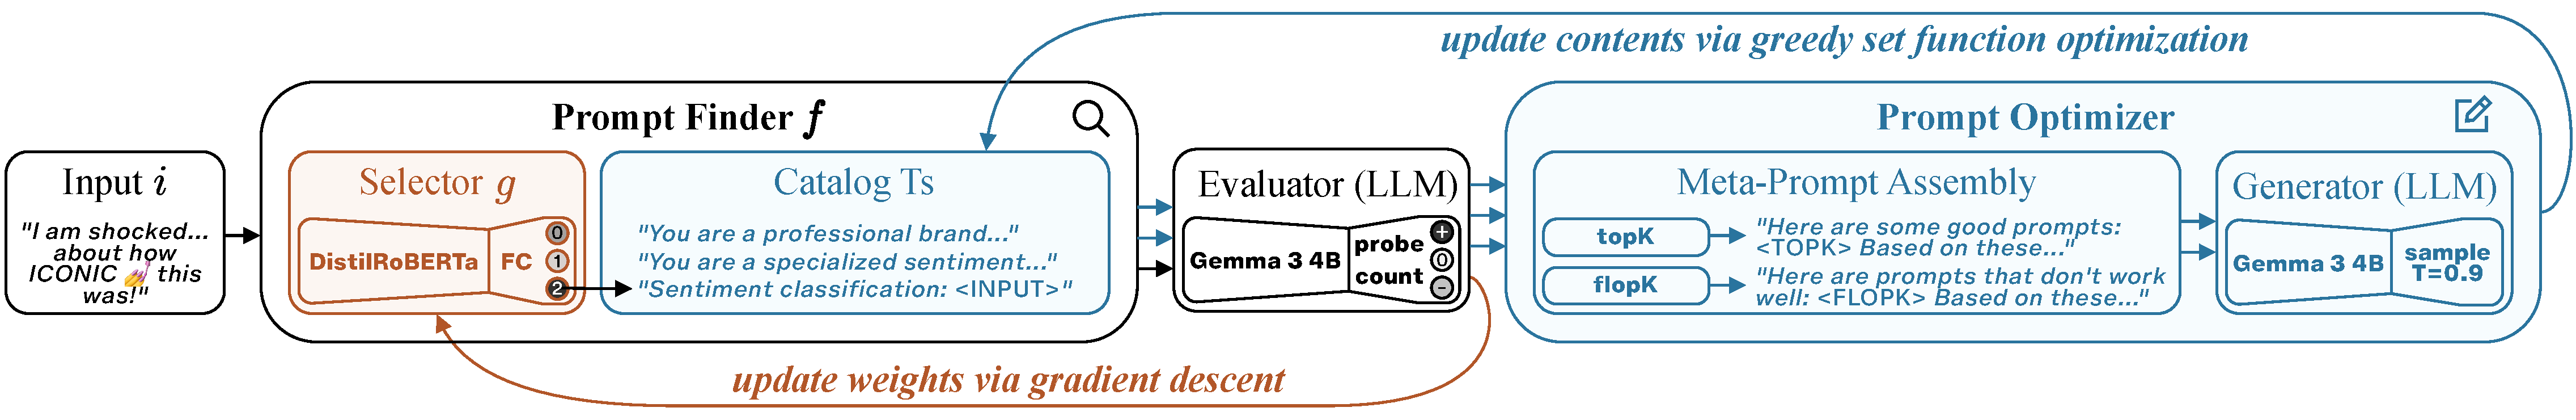
\includegraphics[width=\linewidth]{TablesFigures/pipeline.pdf}
    \vspace{-3ex}
    \caption{An overview of our pipeline combining all methods covered in Section \ref{sec:methods}. The \textcolor{ourorange}{selector (orange)} and \textcolor{ourblue}{catalog (blue)} are optimized separately. At inference time, data only flows along the black path, and the prompt optimizer is disabled.}
    \label{fig:pipeline}
\end{figure*}


This section motivates and specifies each stage of our pipeline in isolation. Denote the classifiable sentiments as $\mathcal{S} := \{\texttt{+}, \texttt{-}, \texttt{0}\}$ and the tokenizer's vocabulary as $\mathcal V$. In line with the definition of the Kleene Star, denote as $\mathcal{V}^*$ the set of all possible sentences.

In our work, a prompt is a tuple $(t, e, M)\in\mathcal T$ of string template $t\in (\mathcal{V}\cup\{\textsc{Input}\})^*$, evaluation strategy $e\in\{\textsc{Probe}, \textsc{Count}\}$, and sentiment map $M \subset {V}^* \times \mathcal{S}$.

How an LLM derives sentiments from prompt-input pairs is detailed in Algorithm \ref{alg:PromptEvaluator}. The evaluation strategy \textsc{Probe} is deterministic and infers probabilities from the \textit{LLM}'s logits. \textsc{Count} is generative and derives probabilities from the number of occurrences of mapped phrases.

\begin{algorithm}[h]
\KwIn{prompt $p=(t,e,M)$, classifiable input $i\in\mathcal{V}^*$}
\KwOut{\{$P[i \text{ has sentiment } s] \mid s\in\mathcal{S}\}$ under $p$}

\vspace{1ex}
$t^{i} :=$ $t$ but replacing each occurrence of $\textsc{Input}$ with $i$\\

\vspace{-2ex}
\uIf{$e = \textsc{Probe}$}{
  $(t_1^i, t_2^i, \ldots, t_n^i) := \textit{LLM.tokenize}(t^i)$\;
  
  \For{$(w,\_) \in M$}{
    $(w_1, w_2, \ldots, w_m) := \textit{LLM.tokenize}(w)$\;
    
    $p_w := \prod_{j\in[m]} P[\textit{LLM.next} = w_j \mid \\\textit{LLM.context} = (t_1^i,\ldots, t_n^i, w_1, \ldots, w_{j-1})]$
  }
  \For{$s\in \mathcal{S}$}{
    $p_s := \frac{1}{|\{(w,s)\in M\}|} \sum_{(w,s)\in M} p_w$
  }
  \Return $\left\{ \frac{p_s}{\sum_{s\in\mathcal S} p_s} \mid s\in \mathcal{S} \right\}$
}

\vspace{1ex}
\uElseIf{$e = \textsc{Count}$}{
    $c$ := $\textit{LLM.createCompletion}(t^i)$\;
    
    \For{$(w,\_) \in M$}{
        $o_w := \text{\# of occurrences of $w$ in $c$}$
    }
    \For{$s\in \mathcal{S}$}{
        $o_s := \sum_{(w,s)\in M} o_w$
    }
    \Return $\left\{ \frac{o_s}{\sum_{s\in\mathcal S} o_s} \mid s\in \mathcal{S} \right\}$
}

\vspace{1ex}

\caption{\textsc{PredictSentiment(\textit{LLM})}}
\label{alg:PromptEvaluator}
\end{algorithm}

Rather than fine-tuning LLM weights, we treat models as black boxes and optimize prompts directly. Given input sentence $i\in\mathcal V^\ast$, we seek a function
\begin{center}
    $f : \mathcal{V}^\ast \to \mathcal T$ that minimizes\\
    $\text{CE}(\textsc{PredictSentiment}(\textit{LLM}, f(i), i), s^\ast)$
\end{center}
where CE denotes the cross-entropy loss between predicted sentiment distribution and the one-hot encoded true sentiment $s^\ast\in\mathcal S$.

\subsection{Prompt Selection}
\label{sec:promptSelection}

Since sentences vary in style, tone, and context, we hypothesize that selecting the most appropriate prompt from a heterogeneous catalog can improve classification performance. Given a fixed prompt catalog $\textit{Ts} \subset \mathcal{T}$, we constrain our optimization to:

\begin{center}
    $f \in \{ i \mapsto \textit{Ts}[g(i)] \mid g: \mathcal V^\ast \to [|\textit{Ts}|] \}$
\end{center}

Here, classifier $g$ maps input sentences to indices in the prompt catalog. This classifier can be much simpler and faster to fine-tune than the evaluating LLM itself. For instance, our selection model DistilRoBERTa \cite{distilRoBERTa} has only 82M parameters compared to the 3B parameters of our evaluating LLM Gemma 3B \cite{gemma_2025}. Additionally, freezing the LLM enables caching outputs between training epochs, substantially increasing sample throughput.

Our approach differs from ensemble methods \cite{ensemble} that evaluate all prompts and aggregate their outputs (e.g., averaging probabilities). Instead of broad consensus, we focus on selecting the single most suitable prompt for each input, which we later show achieves better specialization with lower computational cost.

\subsection{Prompt Optimization}
\label{sec:promptOptimization}

Finding well-performing prompts through human authoring is expensive, while brute-force search is computationally intractable. In Algorithm \ref{alg:PromptOptimizer}, we propose a data-driven approach that automatically evolves prompt catalogs.

\begin{algorithm}[h]
\KwIn{initial prompt catalog $\text{Ts}^{(0)}\subset \mathcal T$, top $K\in\mathbb N$, \newline training set $I\subset\mathcal{V}^*\times \mathcal{S}$, target epoch $J\in\mathbb N$}
\KwOut{refined prompt catalog $\text{Ts}^{(J)}$\newline with $|\text{Ts}^{(J)}|=|\text{Ts}^{(0)}|$}
\vspace{1ex}

\For{$j\in [J]$}{
\For{$\text{\normalfont prompt } p\in \text{Ts}^{(k-1)}$}{
\For{$(\text{\normalfont input }i,\text{\normalfont label }s^\ast)\in I$} {
$\text{AE}_i := |s^\ast -^\# \newline \argmax_s \textsc{PredictSentiment}(LLM, p, i)|$
}
$\text{NMAE}_p := 0.5 \cdot (2 - \frac{1}{|\mathrm{Ts}|} \sum_i \text{AE}_i)$
}

$\text{Tn} := $ $K$ new prompts the LLM generated based on the $\topK_p \text{NMAE}_p$ (bad) and $\topK_p (1 - \text{NMAE}_p)$ (good) prompts\;

$\text{Ts}^{(j)} := \emptyset$\;

\While{$|\text{Ts}^{(j)}| < |\text{Ts}^{(j-1)}|$}{

$p_\text{best} := $ $\argmax_{p\in (\text{Tn}\cup\text{Ts}^{(j-1)}) \setminus \text{Ts}^{(j)}}$ accuracy of $\text{Ts}^{(j)} \cup \{ p \}$ on the training set, assuming the best prompt is chosen for each input sentence.\;

$\text{Ts}^{(j)} := \text{Ts}^{(j)} \cup \{ p_\text{best} \}$
}
}
\Return $\text{Ts}^{(J)}$
\caption{\textsc{OptimizePromptCatalog(\textit{LLM})}}
\label{alg:PromptOptimizer}
\end{algorithm}

Starting with human-written prompts inspired by prompt engineering guides (Appendix \ref{basic_prompt_catalog}), our method iteratively improves the catalog. At each iteration, we evaluate all prompts on a training subset, then provide an LLM with the best and worst performers as examples to generate new prompts. To maintain catalog size and encourage novelty, we discard the worst-performing prompts after each generation.

We evaluate catalog performance assuming perfect prompt selection (Section \ref{sec:promptSelection}) to encourage diversity. The operator $-^\#: \mathcal{S} \times \mathcal{S} \to \pm\{0,1,2\}$ used when calculating the absolute error AE penalizes opposite-sentiment misclassifications more than neutral misclassifications. Since maximizing submodular set functions is NP-hard \cite{subsetSelection}, we use a greedy approximation for prompt selection within each iteration.

\section{Evaluation}\label{evaluation}
In our evaluation, we focus on showing the impact that both the prompt selector and the prompt optimizer have on predicting sentiments in our system. We additionally compare prompted learning to two discriminative models.
To carry out experiments on our system, we manually created a standard prompt catalog that includes simple prompts for $10$ areas of expertise (e.g., restaurants, movies, etc.), which can be found in Appendix \ref{basic_prompt_catalog}. The LLM we use for the prompt evaluator and the optimizer is Gemma 3 (4B) \cite{gemma_2025} in its official Q4\_0 quantization. For sampling, we chose the same parameters as Google in their paper.
\subsection{Prompt Selector}\label{prompt_selector}
\begin{table*}[ht]
\centering
\caption{Classification metrics across domains for individual prompts and prompts adaptively chosen by the prompt selector. }
\vspace{2pt}
\begin{adjustbox}{width=\textwidth}
\begin{tabular}{lcccccccccc|c}
\toprule
\textbf{Metric} & \textbf{Customer} & \textbf{Restaurants} & \textbf{Sarcasm} & \textbf{Brand} & \textbf{Context} & \textbf{Prices} & \textbf{Emotion} & \textbf{Movies} & \textbf{Double} & \textbf{General} & \textbf{Selector} \\
& \textbf{Review} & & & \textbf{Monitor} & & & & & \textbf{Negation} & \\
\midrule
NMAE & 0.81 & 0.80 & 0.80 & 0.81 & 0.82 & 0.78 & 0.79 & 0.8 & 0.6 & 0.8 & \textbf{0.84} \\
Accuracy   & 0.66 & 0.65 & 0.65 & 0.67 & 0.68 & 0.61 & 0.64 & 0.66 & 0.60 & 0.66 & \textbf{0.74} \\
F1         & 0.64 & 0.65 & 0.61 & 0.67 & 0.66 & 0.60 & 0.65 & 0.66 & 0.60 & 0.66 & \textbf{0.73} \\
Precision  & 0.69 & 0.66 & 0.70 & 0.68 & 0.73 & 0.64 & 0.66 & 0.68 & 0.64 & 0.68 & \textbf{0.76} \\
Recall     & 0.65 & 0.68 & 0.63 & 0.70 & 0.64 & 0.62 & 0.69 & 0.69 & 0.66 & 0.71 & \textbf{0.74} \\
\bottomrule
\end{tabular}
\end{adjustbox}
\label{table:selector}
\end{table*}

To analyze the impact the prompt selector has on the overall performance of our system, we carried out an experiment to quantify the impact that this augmentation has on our system.
Table \ref{table:selector} shows that choosing the prompt for each sentence adaptively instead of using a unique prompt for all sentences increases the overall performance of the LLM that receives (prompt, sentence) pairs. We see that the best-performing prompt (``Context''), which emphasizes not to put too much importance on single words, still performs significantly worse than the selector variant. A general prompt that does not include domain-specific instructions also performs significantly worse. We thus conclude that adaptively choosing a prompt by the input sequence increases the performance in our setting. \\
\begin{figure}[ht]
  \centering
  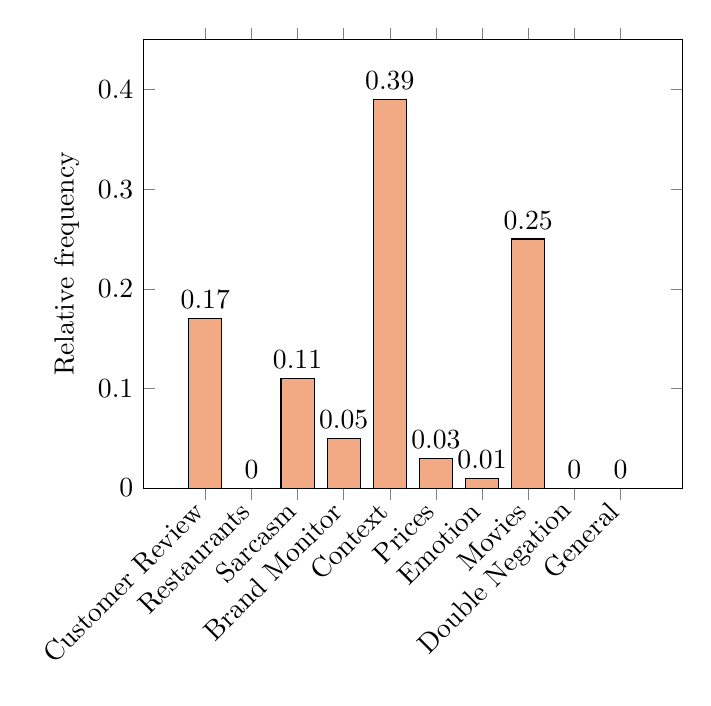
\begin{tikzpicture}
    \begin{axis}[
      ybar,
      bar width=12pt,
      enlarge x limits=0.15,
      ylabel={Relative frequency},
      symbolic x coords={
        Customer Review, Restaurants, Sarcasm, Brand Monitor, Context,
        Prices, Emotion, Movies, Double Negation, General
      },
      xtick=data,
      x tick label style={rotate=45, anchor=east},
      ymin=0,
      ymax=0.45,
      scaled y ticks = false,
      y tick label style={
        /pgf/number format/fixed,
        /pgf/number format/precision=2
      },
      every node near coord/.append style={
        /pgf/number format/fixed,
        /pgf/number format/precision=2
      },
      nodes near coords,
      nodes near coords align={vertical},
    ]
      \addplot[
        fill=customBar,
        draw=black            % or draw=customBar for no border contrast
      ] coordinates {
        (Customer Review,0.17)
        (Restaurants,0.00)
        (Sarcasm,0.11)
        (Brand Monitor,0.05)
        (Context,0.39)
        (Prices,0.03)
        (Emotion,0.01)
        (Movies,0.25)
        (Double Negation,0.00)
        (General,0.00)
      };
    \end{axis}
  \end{tikzpicture}
  \caption{Selection rate of standard prompts by prompt evaluator.}
  \label{fig:selector_freq}
\end{figure}
Figure \ref{fig:selector_freq} shows the relative frequency with which a specific prompt is called. We observed that the selector does not always pick the most successful prompt, but learns to associate specific sentences with the success of specific prompts. For example, by manually inspecting the samples, we saw that movie-related prompts were directed to the movie prompt. \\
In Table \ref{table:optimized}, we see that the evaluator also increased the performance of the optimized prompt catalog.

\subsection{Prompt Optimizer}\label{prompt_optimizer}
In order to quantify the impact of the prompt optimizer on the performance of sentiment analysis in LLMs, we chose to measure the performance of the system with and without prompt optimization on all prompts individually and with the prompt selector activated. In each iteration of the prompt optimizer, we chose to create new prompts based on the three best- and worst-performing prompts of the previous iteration. We conducted our experiments on three iterations, which we deemed a sensible number, given the observations we made in the changes to the prompt catalog. The proper ablation of the number of iterations is up for future work. The updated prompt catalog after three iterations can be found in Appendix \ref{optimized_prompt_catalog}. The meta-prompt used with the optimizing LLM is stated in Appendix \ref{optimizer_prompt}. We observed that prompts generated from poorly performing prompts tended to outperform those derived from well-performing ones.
Table \ref{table:optimized} shows that the best prompt in the standard catalog (``Context'') is still the best in the optimized prompt catalog. We observe that, on the other hand, the mean over the evaluation of the individual prompts goes down by a small margin. This indicates that the prompts on their own perform worse.
This was expected, since we did not train for individually good prompts but for a strong ensemble of prompts. This aligns with the observation that the selector on the optimized prompts performs better than the selector on the standard prompts. Because the improvement is only marginal, we cannot confidently state that there is a significant improvement over the standard catalog.
\begin{table}[ht]
\centering
\caption{Performance metrics for prompting strategies evaluated over all sentences. Single Best uses the one best prompt from the catalog (for all inputs), Mean uses all prompts and takes the mean over their decisions, Selected chooses the prompt adaptively according to the prompt selector's classification.}
\vspace{2pt}
\begin{adjustbox}{width=\columnwidth}
\begin{tabular}{lccc ccc}
\toprule
& \multicolumn{3}{c}{\textbf{Standard Prompts}} & \multicolumn{3}{c}{\textbf{Optimized Prompts}} \\
\cmidrule(lr){2-4} \cmidrule(lr){5-7}
\textbf{Metric}             & \textbf{Single Best} & \textbf{Mean} & \textbf{Selected} & \textbf{Single Best} & \textbf{Mean} & \textbf{Selected} \\
\midrule
NMAE                         & 0.82          & 0.80         & 0.84              & 0.82          & 0.79          & \textbf{0.86}
\\
Accuracy                     & 0.68          & 0.65         & 0.74              & 0.68          & 0.64          & \textbf{0.76}               \\
F1                           & 0.66          & 0.64         & 0.73              & 0.66          & 0.63          & \textbf{0.74}               \\
Precision                    & 0.73          & 0.67         & \textbf{0.76}              & 0.73          & 0.68          & \textbf{0.76}               \\
Recall                       & 0.64          & 0.67         & \textbf{0.74}              & 0.64          & 0.66          & \textbf{0.74}               \\
\bottomrule
\end{tabular}
\end{adjustbox}
\label{table:optimized}
\end{table}

\subsection{Comparison to Discriminative Models}
Discriminative language models such as BERT have been shown to perform well in sentiment analysis \cite{roberta} \cite{discriminativeMullick}. That is why we conducted an analysis to show how learned prompting compares with two end-to-end fine-tuned variants of BERT \cite{bert}, namely DeBERTa \cite{deberta} and RoBERTa \cite{roberta}. Table \ref{table:finetune} shows that DeBERTa performs the best, followed by RoBERTa and our system. We expect those results to improve significantly by using a larger LLM, which we could not utilize due to hardware limitations.

\begin{table}[ht]
\centering
\caption{Comparison of discriminative models vs. learned prompting (DeBERTa selected for Kaggle submission).}
\vspace{2pt}
\begin{adjustbox}{width=\columnwidth}
\begin{tabular}{lccc}
\toprule
\textbf{Metric}               & \textbf{DeBERTa} & \textbf{RoBERTa} & \textbf{Selector \& Optimizer} \\
\midrule
NMAE                          & \textbf{0.89}           & 0.87           & 0.86                        \\
Accuracy                      & \textbf{0.81}           & 0.78           & 0.76                        \\
Precision (macro)             & \textbf{0.81}           & 0.77          & 0.74                         \\
Recall (macro)                & \textbf{0.81}         & 0.78          & 0.76                         \\
F1 (macro)                    & \textbf{0.81}           & 0.78          & 0.74                         \\
\bottomrule
\end{tabular}
\end{adjustbox}
\label{table:finetune}
\end{table}

\section{Conclusion}
% In conclusion, we propose a prompt optimization pipeline that improves the performance of the Gemma 3 (4B) \cite{gemma_2025} large language model on the sentiment analysis of natural language. Our evaluation showed that dynamically choosing the best-fitting prompt based on the input significantly improved the accuracy of sentiment analysis compared to using a static prompt. Furthermore, we found that optimizing the prompt catalog using our prompt optimizer, by generating new prompts based on performance, further improved the accuracy when used in combination with the selector, even though the improvement is moderate.
% We noticed that prompts generated from under-performing prompts generally performed better than those generated from already strong prompts. However, individual optimized prompts did not outperform the best hand-crafted prompts, which indicates that our method is best suited for building a strong ensemble of prompts in the catalog. 
% In general, our evaluation shows that prompt optimization and selection is an effective method to improve LLM performance in natural language sentiment analysis. 
% In future work, we see potential to investigate the behavior of the prompt optimizer further, as this could improve the accuracy of our method even more. 

This work investigated whether learned prompting could serve as a viable alternative to expensive fine-tuning for sentiment analysis via LLMs. Our central hypothesis was that adaptive prompt selection would significantly outperform static prompting by better matching prompt specificity to input characteristics.
Our results strongly support this hypothesis. The prompt selector achieved substantial improvements over all baseline approaches, including the best individual hand-crafted prompts and ensemble methods. This indicates that \textbf{the more specific the prompt, the better the language model performs}, provided specificity is appropriately matched to input rather than applied uniformly.

While individual optimized prompts did not consistently outperform hand-crafted ones, the prompt optimizer created more effective ensembles when combined with the selector. Interestingly, prompts generated from poorly performing examples often outperformed those derived from well-performing ones.
Our approach achieved competitive performance with fine-tuned discriminative models (DeBERTa, RoBERTa) while requiring training only for a lightweight 82M parameter selector—orders of magnitude smaller than fine-tuning the 4B parameter LLM itself. This demonstrates that \textbf{learned prompting represents a computationally efficient alternative to fine-tuning for sentiment analysis}, with important implications for resource-constrained deployments where fine-tuning is impractical.

\bibliography{bibliography}
\bibliographystyle{icml2024}


%%%%%%%%%%%%%%%%%%%%%%%%%%%%%%%%%%%%%%%%%%%%%%%%%%%%%%%%%%%%%%%%%%%%%%%%%%%%%%%
%%%%%%%%%%%%%%%%%%%%%%%%%%%%%%%%%%%%%%%%%%%%%%%%%%%%%%%%%%%%%%%%%%%%%%%%%%%%%%%
% APPENDIX
%%%%%%%%%%%%%%%%%%%%%%%%%%%%%%%%%%%%%%%%%%%%%%%%%%%%%%%%%%%%%%%%%%%%%%%%%%%%%%%
%%%%%%%%%%%%%%%%%%%%%%%%%%%%%%%%%%%%%%%%%%%%%%%%%%%%%%%%%%%%%%%%%%%%%%%%%%%%%%%

\appendix
\section{Prompt Catalog}
\subsection{Standard Prompt Catalog}
\label{basic_prompt_catalog}
In our experiments, we used a manually crafted prompt catalog that are short and simple in their nature but cover various domains and topics. We also included a general prompt to ensure that the other prompts did not perform worse just because they are domain specific. The following list constitutes the standard prompt catalog, ordered by their respective score on the validation set:

\begin{enumerate}
\item You are a highly skilled sentiment analysis expert specializing in analyzing online customer reviews for e-commerce businesses. Categorize it as definitively either positive, negative, or neutral.
\item You are a highly experienced sentiment analysis expert specializing in analyzing online reviews of restaurants. Provide a concise sentiment classification – “positive”, “negative”, or “neutral”. Do not include any explanations or justifications; simply state the sentiment.
\item Sentiment classification task. There can be some sarcasm — pay attention to this. Choose one of the following: positive, negative, or neutral.
\item You are a professional brand monitor tasked with assessing customer feedback. Your role is to categorize the sentiment of each review as either positive, negative, or neutral. Your response MUST be limited to a single word: positive, negative, or neutral. Prioritize accuracy above all else.
\item Sentiment classification task. Don’t let yourself be influenced by single words too much. Analyze the sentence as a whole. Choose carefully one of the following: positive, negative, or neutral.
\item You are a highly experienced sentiment analysis expert specializing in analyzing whether people find prices appropriate. Provide a concise sentiment classification – “positive”, “negative”, or “neutral”. Do not include any explanations or justifications; simply state the sentiment.
\item Do a sentiment classification task. Specialize on people's emotions such as anger or joy. Provide a concise sentiment classification – “positive”, “negative”, or “neutral”. Do not include any explanations or justifications; simply state the sentiment.
\item You are a highly skilled sentiment analysis expert. You will receive reviews about movies. Answer with one word: 'positive', 'negative', or 'neutral'.
\item You are a highly skilled sentiment analysis expert. Focus on double negations in sentences. Answer with one word: 'positive', 'negative', or 'neutral'.
\item You are a highly skilled sentiment analysis expert. Your task is to read sentences and determine the sentiment expressed. The sentiment should be classified as either 'positive', 'negative', or 'neutral'. Provide only the single word sentiment classification.
\end{enumerate}

\subsection{Optimized Prompt Catalog}
\label{optimized_prompt_catalog}
The following list contains the optimized prompts that the optimizer returned ordered by score. Note that some of the prompts remain in the optimized catalogue.
\begin{enumerate}
  \item Sentiment classification task. Don’t let yourself be influenced by single words too much. Analyze the sentence as a whole. Choose carefully one of the following: positive, negative, or neutral.
  \item You are a sentiment analysis expert tasked with classifying the sentiment expressed in customer reviews. Your output should be strictly limited to one of three sentiments: positive, negative, or neutral. Carefully consider the nuances of the text, paying close attention to word choice, context, and any potential sarcasm or irony. When reviewing a sentence, determine if the overall impression conveyed is predominantly positive, negative, or neutral. If the review contains contradictory statements or lacks a clear sentiment, classify it as neutral. If the review expresses a clear liking or disapproval, classify it accordingly. If the review is factual and does not convey an opinion, classify it as neutral. If the review contains both positive and negative elements, determine which sentiment is dominant and classify accordingly. Avoid making assumptions or providing justifications for your classification; simply state the sentiment directly.
  \item You are a professional brand monitor tasked with assessing customer feedback. Your role is to categorize the sentiment of each review as either positive, negative, or neutral. Your response MUST be limited to a single word: positive, negative, or neutral. Prioritize accuracy above all else.
  \item You are a specialized sentiment analyst focused on evaluating online forum discussions related to technology products. Your task is to determine the overall sentiment expressed in each forum post, categorizing it exclusively as positive, negative, or neutral. Carefully scrutinize the text, giving paramount importance to the cumulative impression conveyed rather than focusing on individual words or phrases. Recognize that sarcasm, subtle criticisms, or expressed frustrations can significantly alter the apparent sentiment. Pay particular attention to the tone and language used, considering the context of a technology discussion – often characterized by technical jargon, feature requests, and complaints about bugs or usability issues. If a post primarily describes a factual aspect of a product without any discernible emotional coloring, classify it as neutral. When encountering mixed sentiments—expressed both positive and negative aspects—determine which dominant sentiment prevails and assign the post to that category. Your response should be a
  \item You are a highly specialized sentiment analysis consultant focused exclusively on evaluating feedback related to software development projects. Your task is to determine the overall sentiment expressed in each review and categorize it as either positive, negative, or neutral. Carefully analyze the entire statement, considering the context of software development terminology, potential frustrations with bugs, feature requests, or technical discussions. Pay close attention to phrasing that indicates satisfaction, dissatisfaction, or lack of opinion. Ignore individual words that might appear positive or negative in isolation; instead, assess the holistic impression conveyed. If the review presents a balanced perspective with both positive and negative elements, determine which overarching sentiment is dominant and classify accordingly. When encountering ambiguity or a lack of clear sentiment, categorize the review as neutral. Your response should be limited to a single word: positive, negative, or neutral. Do not provide any explanations or justifications for
  \item You are a highly experienced sentiment analysis expert specializing in analyzing online reviews of restaurants. Provide a concise sentiment classification – “positive”, “negative”, or “neutral”. Do not include any explanations or justifications; simply state the sentiment.
  \item You are a highly skilled sentiment analysis expert. You will receive reviews about movies. Answer with one word: 'positive', 'negative', or 'neutral'.
  \item You are a highly skilled sentiment analysis expert. Your task is to read sentences and determine the sentiment expressed. The sentiment should be classified as either 'positive', 'negative', or 'neutral'. Provide only the single word sentiment classification.
  \item You are a highly skilled sentiment analysis expert. Focus on double negations in sentences. Answer with one word: 'positive', 'negative', or 'neutral'.
  \item You are a seasoned sentiment analysis specialist specializing in analyzing customer reviews for e-commerce platforms. Your task is to carefully examine each provided review and determine its overall sentiment. The output should be negative, positive, or neutral, reflecting your expert judgment considering the entire text. Pay meticulous attention to the language used, including word choice, phrasing, and any subtle indicators of emotion or opinion. Specifically, prioritize identifying sarcasm, irony, implied criticism, and positive sentiment disguised as neutral statements. Consider the context of the review, paying particular attention to the reviewer’s stated goals and expectations. If a review presents a blend of positive and negative aspects, determine the *dominant* sentiment—the one that most accurately captures the reviewer's core feeling. For example, a review stating “The item arrived quickly, but the packaging was damaged” should be categorized as negative.
\end{enumerate}

\section{Prompt Optimizer}
\label{optimizer_prompt}
\subsection{Optimizer Prompt for Top-$k$ Prompts}
We used the following prompt to improve well performing prompts:

\textit{Here are some really good prompts: [WELL\_PERFORMING\_PROMPTS]. Based on these, suggest exactly 1 new prompt templates in a similar style. The goal is to always generate a prompt that can distinguish sentiments of a review as either postive, negative, or neutral. You will want to generate long prompts, that are very specific. Always include as a first sentence in your prompt that the output should be negative, positive or neutral, nothing more. Do not put brakets in your output or any special characters in there, just natural language. Your prompt should not work on all inputs, but very well on a certain type of inputs. So try to produce expert prompts for certain reviews. For example this sentence: 'I highly recommend any location but his.' should be classified as negative. This sentence:'They are just as good at 'soft skills' as translating.' should be classified as positive. Only output the new prompt, nothing else. Avoid at all cost to output anything else than the plain prompt. That means no prefix or suffix.}

\subsection{Optimizer Prompt for Flop-$k$ Prompts}
We used the following prompt to improve poorly performing prompts:

\textit{Here are some prompts that don't work well: [POORLY\_PERFORMING\_PROMPTS]. Based on these, suggest exactly 1 improved prompt templates, that could work better. The goal is to always generate a prompt that can distinguish sentiments of a review as either postive, negative, or neutral. You will want to generate long prompts, that are very specific. Always include as a first sentence in your prompt that the output should be negative, positive or neutral, nothing more. Do not put brakets in your output or any special characters in there, just natural language. Your prompt should not work on all inputs, but very well on a certain type of inputs. So try to produce expert prompts for certain reviews. For example this sentence: 'I highly recommend any location but his.' should be classified as negative. This sentence: They are just as good at 'soft skills' as translating.' should be classified as positive. Only output the new prompt, nothing else. Avoid at all cost to output anything else than the plain prompt. That means no prefix or suffix.}


\end{document}

